% \usetikzlibrary{mindmap,backgrounds}
% \usetikzlibrary{decorations.pathmorphing}
% \usetikzlibrary{decorations.markings}
% \usetikzlibrary{arrows.meta,bending}

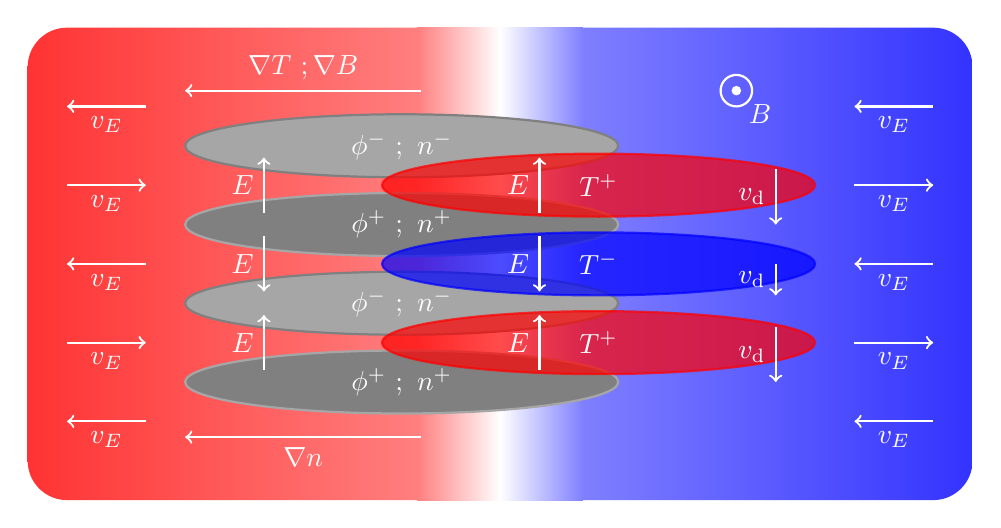
\begin{tikzpicture}

    % Temperature background
    % \shade [left color=red, right color= white, rounded corners = 0cm] (0,0) rectangle (6,6);
    % \shade [left color=white, right color= blue, rounded corners = 0cm] (6,0) rectangle (12,6);

    \onslide<2->{
    \shade [left color=red!80!white, right color= red!50!white]  (5,0) {[rounded corners=0.5cm] --++ (-5,0)  --++ (0,6)} --++ (5,0)  -- cycle;
    \shade [left color=red!50!white, right color= white] (4.95,0) --++ (1.05,0)  --++ (0,6) --++ (-1.05,0)  -- cycle;

    \shade [left color=blue!50!white, right color= blue!80!white]  (7,0) {[rounded corners=0.5cm] --++ (5,0)  --++ (0,6)} --++ (-5,0)  -- cycle;
    \shade [left color=white, right color= blue!50!white] (6,0) --++ (1.05,0)  --++ (0,6) --++ (-1.05,0)  -- cycle;

    }

    \onslide<7->{
    % Density and Potencial cells
    \draw [thick, gray, opacity=1, fill = gray!70!white] (4.75,4.5) ellipse (2.75 and 0.4) node[white, opacity=1]{$\phi^{-}~;~n^{-}$};
    \draw [thick, gray!70!white, opacity=1, fill = gray] (4.75,3.5) ellipse (2.75 and 0.4) node[white, opacity=1]{$\phi^{+}~;~n^{+}$};
    \draw [thick, gray, opacity=1, fill = gray!70!white] (4.75,2.5) ellipse (2.75 and 0.4) node[white, opacity=1]{$\phi^{-}~;~n^{-}$};
    \draw [thick, gray!70!white, opacity=1, fill = gray] (4.75,1.5) ellipse (2.75 and 0.4) node[white, opacity=1]{$\phi^{+}~;~n^{+}$};
    }

    \onslide<4->{
    % Temperature cells
    \draw [thick, red, opacity=0.7, fill = red]   (7.25,4) ellipse (2.75 and 0.4) node[white, opacity=1]{$T^{+}$};
    \draw [thick, blue, opacity=0.7, fill = blue] (7.25,3) ellipse (2.75 and 0.4) node[white, opacity=1]{$T^{-}$};
    \draw [thick, red, opacity=0.7, fill = red]   (7.25,2) ellipse (2.75 and 0.4) node[white, opacity=1]{$T^{+}$};
    }

    \onslide<3->{
    % Temperature and magnetic field gradient
    \draw[thick, white, <-] (2,5.2) -- (5,5.2) node[midway, above, white]{$\nabla T~;\nabla B$};

    % Magnetic field
    \draw [thick, white] (9,5.2) circle (0.2);
    \filldraw [white] (9,5.2) circle (1.5pt);
    \draw (9.3,4.9) node[white]{$\vect{B}$};
    }

    \onslide<6->{
    % Density gradient
    \draw[thick, white, <-] (2,0.8) -- (5,0.8) node[midway, below, white]{$\nabla n$};
    }

    \onslide<8->{
    % Electric field
    \draw[thick, white, <-] (3,4.35) -- (3,3.65) node[midway, below, left]{$\vect{E}$};
    \draw[thick, white, <-] (6.5,4.35) -- (6.5,3.65) node[midway, below, left]{$\vect{E}$};
    \draw[thick, white, ->] (3,3.35) -- (3,2.65) node[midway, below, left]{$\vect{E}$};
    \draw[thick, white, ->] (6.5,3.35) -- (6.5,2.65) node[midway, below, left]{$\vect{E}$};
    \draw[thick, white, <-] (3,2.35) -- (3,1.65) node[midway, below, left]{$\vect{E}$};
    \draw[thick, white, <-] (6.5,2.35) -- (6.5,1.65) node[midway, below, left]{$\vect{E}$};
    }

    \onslide<5->{
    % Grad B and curvature drift velocity
    \draw[thick, white, ->] (9.5,4.2) -- (9.5,3.5) node[midway, left, white]{$\vect{v}_\mathrm{d}$};
    \draw[thick, white, ->] (9.5,3)   -- (9.5,2.6) node[midway, left, white]{$\vect{v}_\mathrm{d}$};
    \draw[thick, white, ->] (9.5,2.2) -- (9.5,1.5) node[midway, left, white]{$\vect{v}_\mathrm{d}$};
    }

    \onslide<9->{
    % ExB drift velocity
    \draw[thick, white, <-] (10.5,5) -- (11.5,5) node[midway, below, white]{$\vect{v}_{E}$};
    \draw[thick, white, ->] (10.5,4) -- (11.5,4) node[midway, below, white]{$\vect{v}_{E}$};
    \draw[thick, white, <-] (10.5,3) -- (11.5,3) node[midway, below, white]{$\vect{v}_{E}$};
    \draw[thick, white, ->] (10.5,2) -- (11.5,2) node[midway, below, white]{$\vect{v}_{E}$};
    \draw[thick, white, <-] (10.5,1) -- (11.5,1) node[midway, below, white]{$\vect{v}_{E}$};
    \draw[thick, white, <-] (0.5,5)  --  (1.5,5) node[midway, below, white]{$\vect{v}_{E}$};
    \draw[thick, white, ->] (0.5,4)  --  (1.5,4) node[midway, below, white]{$\vect{v}_{E}$};
    \draw[thick, white, <-] (0.5,3)  --  (1.5,3) node[midway, below, white]{$\vect{v}_{E}$};
    \draw[thick, white, ->] (0.5,2)  --  (1.5,2) node[midway, below, white]{$\vect{v}_{E}$};
    \draw[thick, white, <-] (0.5,1)  --  (1.5,1) node[midway, below, white]{$\vect{v}_{E}$};
    }

\end{tikzpicture}